% !TeX spellcheck = en_US
\documentclass[a4paper]{article}
\usepackage[utf8]{inputenc}
%\usepackage{a4}
\usepackage{graphicx}
\graphicspath{/pictures}
\sloppy
\usepackage{parskip} %Make a new line in pdf 
\usepackage{hyperref} %Quick links
%\usepackage[ngerman]{babel}
\renewcommand*\rmdefault{ppl} %Schrift
\usepackage{listings}
\usepackage{color}
\usepackage{tikz}
\usepackage{pgfplots}
\usepackage{pgfplotstable}
\usepackage{float}
\usepackage{graphicx}
\usepackage{caption}
\usepackage{subcaption}

\usepackage{etoolbox}
%\usepackage{showframe}
\makeatletter
\patchcmd{\@makechapterhead}{\vspace*{50\p@}}{}{}{}% Removes space above \chapter head
\patchcmd{\@makeschapterhead}{\vspace*{50\p@}}{}{}{}% Removes space above \chapter* head
\makeatother

\definecolor{listinggray}{gray}{0.9}
\definecolor{lbcolor}{rgb}{0.9,0.9,0.9}
%Adapted from http://tex.stackexchange.com/questions/81834/whats-the-best-way-to-typeset-c-codes-in-latex
\lstset{
	tabsize=4,    
	language=[GNU]C++,
	basicstyle=\scriptsize,
	upquote=true,
	aboveskip={1.5\baselineskip},
	columns=fixed,
	showstringspaces=false,
	extendedchars=false,
	breaklines=true,
	prebreak = \raisebox{0ex}[0ex][0ex]{\ensuremath{\hookleftarrow}},
	frame=none,
	numbers=left,
	showtabs=false,
	showspaces=false,
	showstringspaces=false,
	identifierstyle=\ttfamily,
	keywordstyle=\color[rgb]{0,0,1},
	commentstyle=\color[rgb]{0.026,0.112,0.095},
	stringstyle=\color[rgb]{0.627,0.126,0.941},
	numberstyle=\color[rgb]{0.205, 0.142, 0.73},
	%        \lstdefinestyle{C++}{language=C++,style=numbers}’.
}

\newcommand{\td}[1]{
	\textbf{\color{red}TODO: {#1}}
}


\makeatletter
\pgfplotsset{
	/pgfplots/flexible xticklabels from table/.code n args={3}{%
		\pgfplotstableread[#3]{#1}\coordinate@table
		\pgfplotstablegetcolumn{#2}\of{\coordinate@table}\to\pgfplots@xticklabels
		\let\pgfplots@xticklabel=\pgfplots@user@ticklabel@list@x
	}
}
\makeatother

\newcommand{\createPlot}[3]{
	\scriptsize
	\begin{tikzpicture}
	\pgfplotstableread[col sep=comma]{#1}\datatable
	\begin{axis}[
	ybar, ymin=0,
	xlabel={#2},
	ylabel=Time in s,
	%ymode=log,
	ymajorgrids,
	flexible xticklabels from table={#1}{{#2}}{col sep=comma},
	xticklabel style={rotate=45, anchor=east, align=right,text width=1.0cm},
	xtick=data,
	nodes near coords align={vertical}]
	\addplot[blue!20!black,fill=blue!50!white] table[x expr=\coordindex,y={#3}]{\datatable};
	
	\end{axis}
	\end{tikzpicture}\\
	
}




\begin{document}


\begin{center}
	\huge\textbf{Solution Worksheet 2}\\
	\bigskip
	\normalsize Vishal Sontakke, Felix Späth, Michael Zellner, Christopher Zöller
	
\end{center}


\section{Parallelization}

We implemented the MPI\_Communication via MPI\_Datatypes. Our datatypes are the following ones:

\begin{lstlisting}
	MPI_Datatype _pres_right;  MPI_Datatype _pres_left;
	MPI_Datatype _pres_top;    MPI_Datatype _pres_bottom;
	MPI_Datatype _pres_front;  MPI_Datatype _pres_back;
	
	MPI_Datatype _velo_right;  MPI_Datatype _velo_left;
	MPI_Datatype _velo_top;    MPI_Datatype _velo_bottom;
	MPI_Datatype _velo_front;  MPI_Datatype _velo_back;
\end{lstlisting}

The definition of the datatypes are for example the following ones (in 2D):
\begin{lstlisting}

MPI_Type_vector(y, 
				1, 
				x+3, 
				MY_MPI_FLOAT,
				&_pres_left
				);

MPI_Type_vector(y,
				2, 
				x+3, 
				MY_MPI_FLOAT,	
				&_pres_right
				);
\end{lstlisting}

By defining the datatypes like this it is not necessary to fill and read the pressure and velocity buffers. Additionally, an iterator is not necessary anymore.


\subsection{Communication of Flow Quantities}
\begin{itemize}
	\item \textbf{Check out the implementation of the iterator ParallelBoundaryIterator.}\\
	Done.
	\item \textbf{Read the implementation and infer its functional meaning: which cells does the iterator operate on?}\\
	The iterator will move over the boundary layer if there is a neighboring rank available. For each cell it applies a BoundaryStencil. One can specify an offset so it can iterate over inner cells.
	\newpage
	\item \textbf{Which functions does a respective stencil object need to provide?}\\
	The following functions are necessary because they are defined as virtual.
	\begin{lstlisting}
	void applyLeftWall   (FlowField & flowField, int i, int j);
	void applyRightWall  (FlowField & flowField, int i, int j);
	void applyBottomWall (FlowField & flowField, int i, int j);
	void applyTopWall    (FlowField & flowField, int i, int j);
	void applyLeftWall   (FlowField & flowField, int i, int j, int k);
	void applyRightWall  (FlowField & flowField, int i, int j, int k);
	void applyBottomWall (FlowField & flowField, int i, int j, int k);
	void applyTopWall    (FlowField & flowField, int i, int j, int k);
	void applyFrontWall  (FlowField & flowField, int i, int j, int k);
	void applyBackWall   (FlowField & flowField, int i, int j, int k);
	\end{lstlisting}
	
	\item \textbf{Can you reuse existing stencil formats, or are new stencil types required?}\\
	Since every function in BoundaryStencil is virtual we would have to define new ones.
	
	\item \textbf{Implement a boundary stencil PressureBufferFillStencil which reads the pressure values in each of the six (3D) boundary faces of a sub-domain (i.e. the domain of one process) and stores them consecutively in one-dimensional buffer arrays (one array for each of the six faces). For traversal of the respectivesub-domain cells, cf. 1.}\\
	Not necessary because we are using MPI\_Datatypes.
	
	\item \textbf{Implement a boundary stencil PressureBufferReadStencil which reads data from one- dimensional arrays (one array for each of the six faces) and writes them into the correct cells of the boundary.}\\
	Not necessary because we are using MPI\_Datatypes.
	
	\item \textbf{Integrate the read- and write operations into a class PetscParallelManager. The Petsc- ParallelManager should provide a method communicatePressure() (...)}\\
	Our communicatePressure() and communicateVelocity() methods consists of simple MPI\_SendRecv operations. Filling and reading buffer is not necessary because the MPI\_Datatypes will take care of that.
	
	\item \textbf{Implement the exchange of velocities analogously to the steps 1-4. Implement write- and read-stencils VelocityBufferFillStencil and VelocityBufferReadStencil and integrate them into the PetscParallelManager. The respective method communicate- Velocities() should further handle the exchange of the velocity buffers between the processes.}\\
	Done.
	
	\item \textbf{Integrate the PetscParallelManager and respective calls to its communication methods into the class Simulation. Test the exchange of flow quantities in cavity, channel and backward-facing step flows. It is sufficient to only consider the first time step (the choice of a maximum time step should not have severe impact on the testing).}\\
	Done. Tests were executed for 2D and 3D cases on every scenario. 
	
\end{itemize}
\subsection{Global Synchronization of the Time Step}
\begin{itemize}
	\item \textbf{Check out the implementation of setTimeStep() in the class Simulation. How is the maximum time step evaluated in the parallel simulation?}\\
	Each rank computes its minimum timestep afterwards the global minimum is derived from those values. MPI\_Allreduce(...) takes care of the reduction and broadcast.

\end{itemize}

\subsection{Validation}
\begin{itemize}
	\item \textbf{Validate your parallel implementation for different domain decompositions, that is different choices $P_x$ x $P_y$ x $P_z$ , and domain sizes. Use cavity, channel and backward-facing step simulations for this purpose. Compare the solutions to your sequential program. What do you observe?}\\
	Done.\\
	Corner cells need to be send, too. These are needed for the derivatives as they contain the values of their right boarder.
	We tested the dimensional splitting in different 2D and 3D channel flow test-cases, with and without turbulence. The communication works as specified and gives the same results as the sequential code, even the numerical problem in the 3D channel flow is independent from the parallelization. The cavity scenario was tested with 2D and 3D, but without turbulence.
	We observed, that it is hard to achieve a speedup by adding more MPI-ranks as the number of iterations petsc needs increases dramatically, see next chapter for more details.
	
\end{itemize}

\section{Scaling and Efficiency}
\subsection{Theory: Towards Scaling Experiments}
\begin{itemize}
	\item \textbf{How can weak and strong scaling be measured for NS-EOF? Which problems do you expect?}\\
	Strong scaling should be easy to measure by choosing a large scenario. We should be able to increase the number of processors working on the problem in order to achieve a lower execution time.\\
	Weak scaling will be tricky because the number of iterations of PETSC is dependent on the number of cells. The increase of computational work is therefore higher than the increase of cell-count. A good metrics would probably meassure the time per itreation and include this. We will just keep the number of cells per process constant. \\
\end{itemize}
\subsection{NS-EOF in the MAC-cluster}
\subsubsection{Environment and Login}
Done.
\subsubsection{Compiling}
Due to the fact that PETSC is not fully supported by the MAC cluster we compiled our own version for this worksheet. We used the version 3.7.4 the commands to compile it are the following ones:
\begin{lstlisting}[caption=Debug version]
wget http://ftp.mcs.anl.gov/pub/petsc/release-snapshots/petsc-3.7.4.tar.gz
mkdir $HOME/petsc
tar -xvf petsc-3.7.4.tar.gz
cd petsc-3.7.4

#maccluster
python2 ./configure \
--with-blas-lapack-dir=$MKLROOT \
--with-mpi=1 \
--with-mpi-dir=$MPI_BASE  \
--prefix=$HOME/petsc/petsc-3.7.4-debug \
--CC=mpiicc \
--CXX=mpiicpc \
--FC=mpiifort \
--CPPFLAGS="-g -O3" \ # -xHOST does not work with debugging=1
--CFLAGS="-g -O3" \
--CXXFLAGS="-g -O3" \
--with-vendor-compilers=intel \
--known-mpi-shared-libraries=1 \
--with-make-np=28 \
--with-batch=1 \
--with-debugging=1 \ # Set to zero for release version
--PETSC_ARCH=petsc-3-7-4-debug

salloc -n 1 -p snb
cd $HOME/petsc/petsc-3.7.4
./conftest-petsc-3-7-4-release

#[Ctr + D]

./reconfigure-petsc-3-7-4-release.py

make PETSC_DIR=$HOME/petsc-3.7.4 PETSC_ARCH=petsc-3-7-4-release all
make PETSC_DIR=$HOME/petsc-3.7.4 PETSC_ARCH=petsc-3-7-4-release install

#in .bashrc
export LD_LIBRARY_PATH=$LD_LIBRARY_PATH:$HOME/petsc/petsc-3.7.4/lib
export PETSC_DIR=$HOME/petsc/petsc-3.7.4
\end{lstlisting}





\subsubsection{Execution}
Done
\subsection{Scaling Measurements}
\begin{itemize}
	\item \textbf{Choose suitable simulation scenarios for the scaling measurements with respect to domain size, domain decomposition and the flow problem under consideration.}\\
	
	\textbf{Strong scaling results:}

\begin{figure}[H]
	\hspace{-3cm}
	\begin{minipage}{.7\textwidth}
		\centering
		\createPlot{csv/N1IncX.csv}{Processes}{Time}	
		\caption{On one Node with domain size 120x120. Increase number of ranks in x-direction}
	\end{minipage}%
	\begin{minipage}{.8\textwidth}
		\centering
		\createPlot{csv/N1IncY.csv}{Processes}{Time}	
		\caption{On one Node with domain size 120x120. Increase number of ranks in y-direction}
	\end{minipage}
\end{figure}

\begin{figure}[H]
	\centering
	\createPlot{csv/N1IncXY.csv}{Processes}{Time}
	\caption{On one Node with domain size 120x120. Increase number of ranks in x- and y-direction}
\end{figure}


\begin{figure}[H]
	\hspace{-3cm}
	\begin{minipage}{.7\textwidth}
		\centering
		\createPlot{csv/N2.csv}{Processes}{Time}
		\caption{On two Node with domain size 120x120}
	\end{minipage}%
	\begin{minipage}{.8\textwidth}
		\centering
		\createPlot{csv/N4.csv}{Processes}{Time}
		\caption{On four Node with domain size 120x120}
	\end{minipage}
\end{figure}


\textbf{Weak scaling results:}
\begin{figure}[H]
	\centering
	\createPlot{csv/weak.csv}{Processes}{Time}
	\caption{On one node. 40x40 per rank.}
\end{figure}
	
	\item \textbf{Run your parallel simulations for various numbers of processors and architectures. Plot your speedup and parallel efficiency in respective graphs (processes vs. speedup, e.g.). Hint: Deactivate vtk output in the scaling experiments since our output is not optimized for parallel execution yet.}\\
	\td{Out VTK output is per rank. Moreover maybe we should compare binary and ascii output here}
	\item\textbf{How can you improve the performance of your program?}\\
	Since the Petsc part is the most compute intensive one. One should try to improve this. About 65\% of the runtime is spend in Petsc. Probably a better parallelization of this part by using for example OpenMP could help to address this problem. Moreover another Preconditioner could help to decrease the time which is spend in petsc.
	\item\textbf{Optimize your software. You may work on both sequential and parallel improvements as well as on algorithmic optimizations (such as optimization of the pressure Poisson solver).}\\
	One optimization we did was to use a better implementation for the MPI communication. With our MPI\_Datatypes unnecessary fill and read operation on the communication buffers are not a problem anymore. Additionally, our code is much cleaner as before because it is about 500 loc less.
	Another improvement is the BinaryVTK output. It is much faster and safes harddisk space.
\end{itemize}

\section{Turbulence Modeling}
\subsection{Implementation of an algebraic turbulence model}
\begin{itemize}
	\item \textbf{Compute a laminar reference case. Therefore, set $v_T = 0$.}\\
	Done with 2D.\\
	3D has been implemented but there is a bug which we are not able to find out which causes PETSc to diverge after few time steps.
	\item \textbf{Implement the Prandtl mixing length model. Consider that you need to know the local distance to the nearest wall as well as $S_{ij}$.}\\
	Done.
	\item \textbf{Following these instructions,}
	\begin{itemize}
		\item \textbf{experiment two of the four options.}\\
		We chose to implement equation 6 and 7 as well as the option without boundary layer thickness dependency of the mixing length. In the following we will discuss the two models using equation 6 and 7 respectively. 
		\item \textbf{explain your choices. What would you have expected and how does that differ from your findings?}\\
The two equations resolve the evolution of the boundary layer thickness in flow direction which will lead to a more accurate description of the boundary layer development compared to a model where the boundary layer thickness depends solely on the wall normal distance. 
The Blasius boundary layer equation describes a boundary layer thickness which is inverse proportional to the square root of Re\_x whereas the turbulent boundary layer model has the boundary layer thickness proportional to the inverse of the 5th root. We expect those proportionalities will show in the development of the boundary layer thickness and therefore in the mixing length and turbulent viscosity. 
		\item \textbf{discuss your results and compare the results of your two modeling approaches.}\\
The results show the expected proportionalities to the boundary layer thickness functions. Since the Blasisus boundary layer thickness increases faster than the turbulent boundary layer thickness and therefore the turbulent viscosity is higher in the entrance area of the channel. At x/H = 20 both laminar and turbulent boundary layer thickness are larger than kappa*h and therefore both models calculate the same turbulent viscosity. 
		\item \textbf{compare your findings to the laminar reference case.}\\
In the laminar reference case the turbulent viscosity is set to zero which results in less exchange of momentum in the fluid and therefore the velocity gradients are weaker and the maximum velocity is higher.
	\end{itemize}
\end{itemize}
\subsection{Implementational Details}
\subsubsection{Prerequisites}
	\begin{itemize}
	\item \textbf{Extend the configuration of the simulation such that all parameters required by your turbulence model implementation can also be read from the xml-files.}\\
	Done.
\end{itemize}
\subsubsection{Turbulent viscosity and wall distance}
\begin{itemize}
	\item \textbf{Extend the data structures for the turbulent case. In order to keep things simple, you may add a new scalar field for both the distance to the (nearest) wall and a scalar field to store the turbulent viscosity $vT$ . We further evaluate the turbulent viscosity in the cell center, i.e. at the same location as the pressure.}\\
	The turbulent viscosity calculation is implemented in the TurbLPModelStencil files. The Stencil consists of properties for the local velocities and local mesh sizes, the getShearStressTensorProduct which determines the square root in equation (4) and the apply methods that calculate the  turbulent viscosity value for each cell. The derivatives for the shear stress tensor are implemented in the StencilFunctions.h file. The mixing length is stored in TurbFlowField and calculated in MixingLengthStencil. 
	\item \textbf{Consider the basic interplay of stencils, iterators and data structures in NS-EOF. How can you apply the concept of inheritance so that you can naturally extend your data structures and support both old and potentially new data structures in case of turbulence- model-based simulations?}\\
	Done.
	\item \textbf{Implement a VTK visualization for the turbulent viscosity. You may base your implementations on the existing plotter (VTKStencil) for the turbulent case and create a new stencil for this purpose which operates on the new data structure.}\\
	Done.
\end{itemize}

\subsubsection{Momentum equations}
\begin{itemize}
	\item \textbf{Replace the discretization of the Laplacian in the evaluation of F, G and H by discrete expressions for}\\
	The velocity terms F, G and H are being evaluated in TurbFGHStencil. The methods that compute F, G and H are implemented in StencilFunctions. The compute functions used for the DNS simulations are overloaded and the evaluation of the Laplacian is changed to the evaluation of the three summands of equation (8-10) respectively.  The methods used to calculate these summands consist of the derivative-methods and the methods that determine the turbulent viscosity at cell edges. 
	\item \textbf{Improve your implementation by extending it to stretched meshes. How do you need to adapt the formulas for F, G, H from above?}\\
	We extend the implementation to stretched meshes by looking at the cell sizes and weighing the respective cell with the respective ratio. This is similar to what is already implemented in the code for other derivatives.
\end{itemize}

\subsubsection{Parallelization}
\begin{itemize}
	\item \textbf{Extend interprocess communication by communication routines for the viscosity field. The communication of turbulent viscosity is carried out analogously to the communication of the pressure. How can you use the concept of inheritance to extend and reuse the existing communication routines from the PetscParallelManager?}\\
	Done. Similar to the communication of pressure and velocity using MPI\_DATA\_TYPE.
	\item \textbf{Extend the configuration by broadcasting the new parameters to all processes. You may use the methods MPI Bcast(...) and broadcastString(...), provided by MPI and the class Configuration.}\\
	Done.
\end{itemize}
\subsubsection{Plugging things together}
\begin{itemize}
	\item \textbf{Use the concept of inheritance to create a simulation class TurbulentSimulation which possesses all properties of Simulation and incorporates the features of the algebraic turbulence modeling.}\\
	Done.
	\item \textbf{Adapt the time step restriction in TurbulentSimulation. Due to your inhomogeneous viscosity, the original expression for diffusive time step limitations}\\
	Done.
	\item \textbf{Implement the evaluation of the new time step criterion using the stencil-iterator concept.}\\
	Done.
	
	
\end{itemize}





\section{Testing}
\begin{itemize}
	\item \textbf{Test your parallel, turbulent flow simulation code in various channel flow scenarios. How can you verify that all finite difference expressions and parallel extensions are evaluated correctly?}\\
	Running the simulation with turbulent viscosity, $\nu_{T}$, set to 0 if we observe that the output is the same as dns simulation then we conclude that the derivatives are correct. If the derivatives were wrong then we would not see this in the output.

 
	\item \textbf{Experiment with your choices on turbulence models in channel flows (cf. Sec. 3.1). What do you observe? How do the different models behave?}\\
	In the following graph the the normalized velocity profiles of a DNS simulation and a laminar RANS simulation for Re = 1000 are plotted ar x/H = 20 over the dimensionless wall normal distance. The profiles are congruent. Therefore the derivatives must be evaluated correctly. The domain has been decomposed into 4x2 blocks for the parallel compuation. The flow field throughout the channel does not show any unphysical sudden changes in flow properties and single core simulations show the same results. Therefore the parallel extensions are evaluated correctly.\\ 
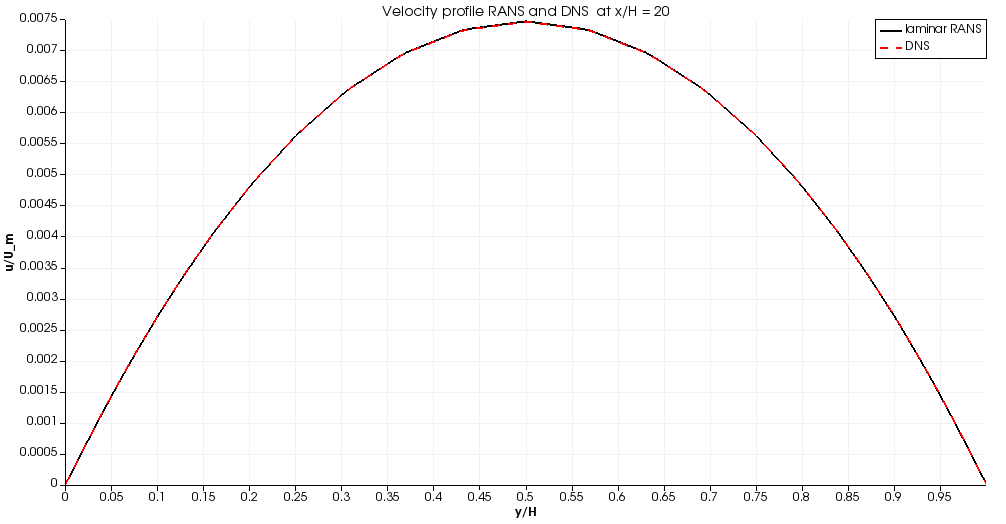
\includegraphics[width=0.9\textwidth]{pictures/1_Velocity_profile_RANS_and_DNS_at_20}\\

The mixing length development in flow direction is in accordance with the x-dependency of the two boundary layer thickness equations. Therefore the mixing length increases faster when the Blasius boundary layer equation is used than it does for the turbulent boundary layer model. The graph below shows the evolution of the mixing length along the center line of the channel. The mixing length increases with the boundary layer thickness until $\kappa$ *h is the restricting factor. \\

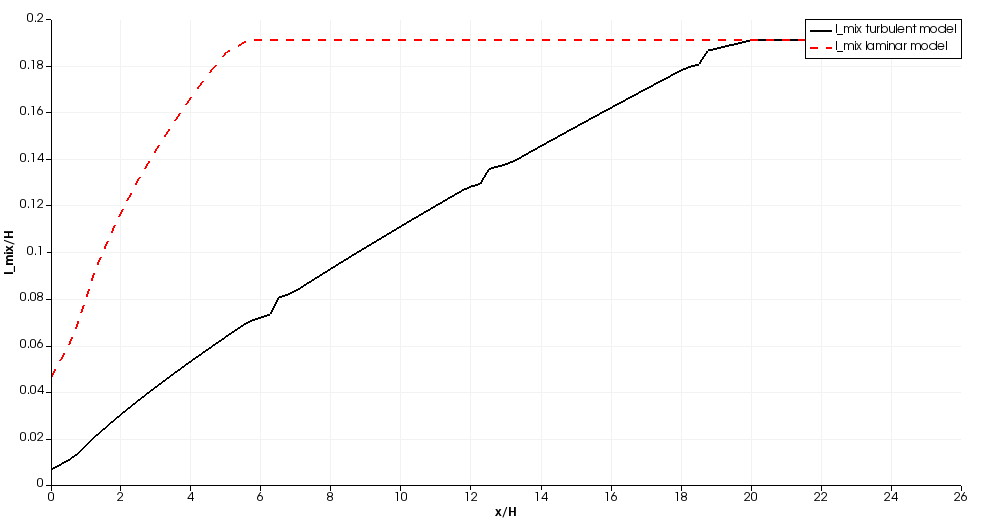
\includegraphics[width=0.9\textwidth]{pictures/2_Mixing_lengths}\\

As the plot of the mixing length development has shown, differences in turbulent viscosity exist only until x/H = 20 is reached. Therefore the velocity profiles at x/H = 20 should be similar for both turbulence models whereas they should differ in the entrance region. This behavior is shown in the following two velocity profile graphs where the velocity profiles are plotted at x/H = 5 and x/H = 20. \\

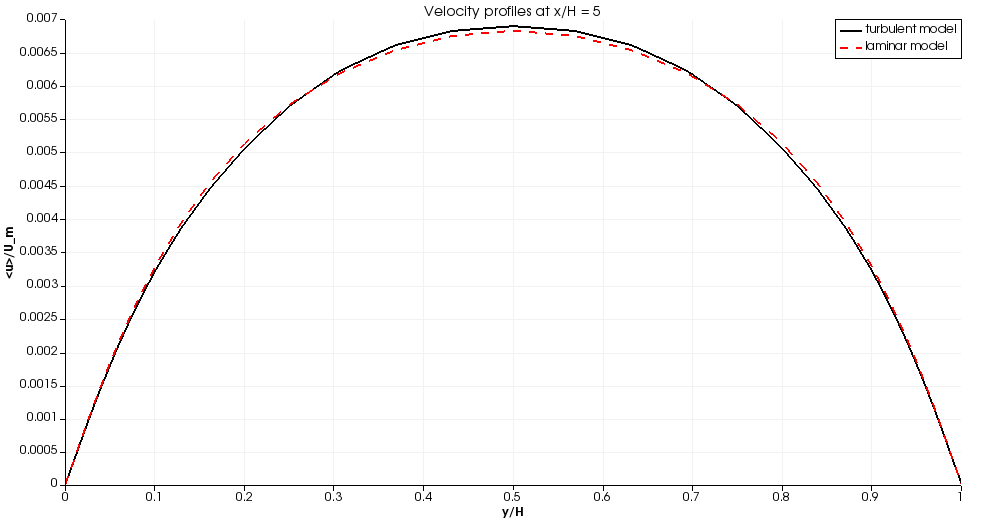
\includegraphics[width=0.9\textwidth]{pictures/2_Velocity_Profile_x5}\\

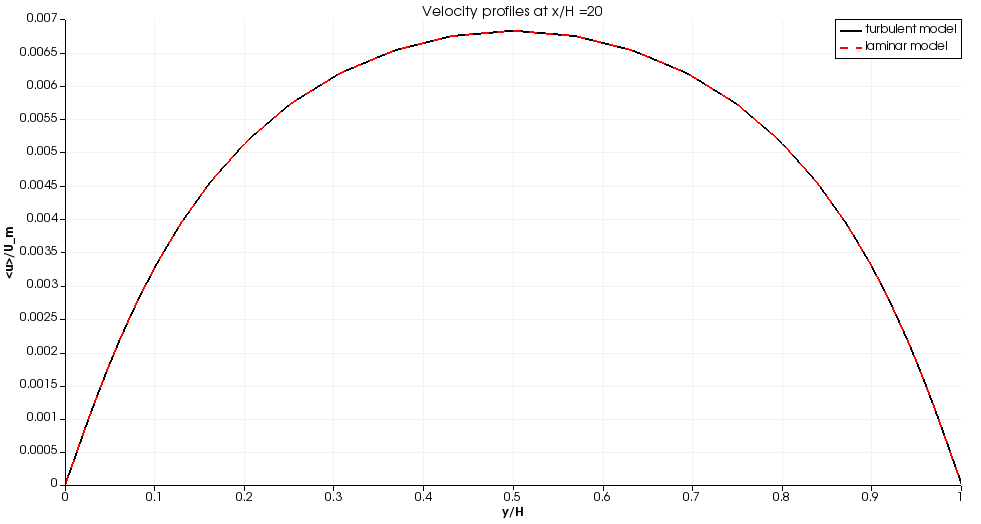
\includegraphics[width=0.9\textwidth]{pictures/2_Velocity_Profile_x20}\\

The following plot shows the production term of the Reynolds stress tensor normalized with the wall shear stress over the normalized wall normal direction. With an increase in the Reynolds number the turbulence production increases. The decay of the turbulence production towards the channel center is not linear as expected. The turbulence production close to the wall is larger than expected. It reaches values close to one, which does not coincide with the results that are found in literature.  We conclude there is an overproduction of turbulence close to the wall. 

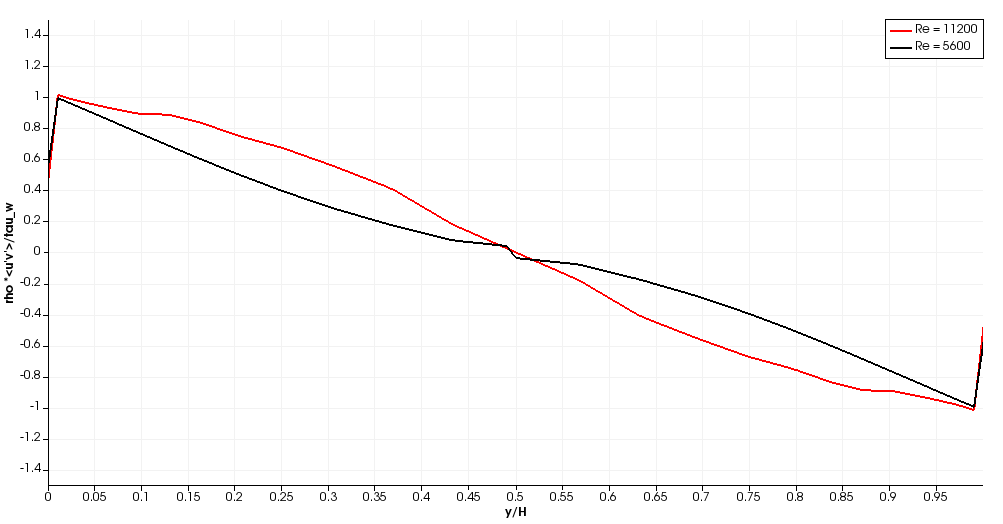
\includegraphics[width=0.9\textwidth]{pictures/Reynolds_Stress_Re5600_Re11200}\\

	\item\textbf{Run turbulence simulations for the backward-facing step scenario.}\\
	\td{}\\
	\td{Attach your discussions and appropriate plots as a pdf-file to the code you submit!}
\end{itemize}





\end{document}
